
\chapter{Matching Condition Code Uses and Definitions}
\label{ch-ccmatch}

{\small
\begin{flushright}
Design: Cristina and Mike [c.99]; Documentation: Mike [17 May 00]; Implementation: Mike
\end{flushright} 
}

% These macros save a bit of typing
\newcommand{\ltu}{$<_u$}    % Unsigned less than
\newcommand{\gtu}{$>_u$}    % Unsigned greater than

This chapter covers the removal of condition codes (CCs) via matching of 
condition code uses with a suitable definition, thereby converting this 
pair into a high level expression that no longer involves a condition code.

The types of instructions that use condition codes are:
\begin{itemize}
\item Conditional branches, e.g. branch on minus.
\item Conditional set instructions, e.g. \texttt{sgt dest} (set \texttt{dest}
to one if signed greater than; else set to zero).
\item Arithmetic instructions, e.g. add with carry. There are two main
    subtypes of these:
\begin{itemize}
    \item Certain idioms, e.g. this one means ``if (a != 0) goto dest'':
    \begin{verbatim}
        cmp  0,a
        addx 0,0,dest
    \end{verbatim}
    [The SPARC addx (add with extend) means add with carry.]
    \item Multiword arithmetic, e.g. adding b:d to a:d (where : means
        concatenation)
    \begin{verbatim}
        add  a,b
        addx c,d
    \end{verbatim}
\end{itemize}
\end{itemize}

The types of instuctions that set condition codes are:
\begin{itemize}
\item Compare instructions, e.g. \texttt{cmp a,b}. These are often (but not
always) paired with conditional branches.
\item Arithmetic instructions, e.g. \texttt{add a,b} and the Pentium
\texttt{bt reg,\#7} (test bit 7 in register \texttt{reg}; copies
that bit to the carry flag).
\end{itemize}

Once a use of a condition code has been matched with its definition, the
resultant \hrtl\ transformations depend on the kinds of instruction using and
defining the condition code. This is covered in detail in
section~\ref{sec-comb-use-def}, but the most common case is that of a
compare instruction (setting the condition code), and a conditional branch
(using the condition code). In this case, the transformations involve setting
one or two variables (depending on the branch) to the operands of the compare,
and setting the high level condition (an expression in the form of a semantic
string) in the high level branch (HLJcond object). For example:

Original instructions:
\begin{verbatim}
10aac:  80 a4 00 08        cmp          %l0, %o0
10ab0:  12 80 00 06        bne          0x10ac8
\end{verbatim}

Low level RTLs (before analysis):
\begin{verbatim}
00010aac *32* r[0] := r[16] - r[8]
         SUBFLAGS( r[16], r[8], r[0] )
00010ab0  JCOND 10ac8, condition not equals
\end{verbatim}

High level RTLs (after analysis):
\begin{verbatim}
00010aac *32* r[0] := r[16] - v2
         *32* v10 := r[0]
         SUBFLAGS( r[16], v2, r[0] )
00010ab0 *32* v2 := 70656       # Delay slot instruction
00010ab0  JCOND 10ac8, condition not equals
High level: v10 ~= 0
\end{verbatim}

The most difficult aspect of eliminating condition codes is the successful
matching of uses with definitions, especially where a use has multiple
definitions, or where a basic block between the use and definition has more
than one in-edge. The basic process used is to scan backwards through the
control flow graph of the procedure from each use of a condition code; see
Figure~\ref{fig-duplicateBB}. In the figure, ``Use'' is a basic block using
a condition code, and the goal is to find BBs like ``Def'' that define that
condition code along a unique path. If a definition is found, the combining
process can begin (see section~\ref{sec-comb-use-def}).
Where there is only one in-edge to a basic block, that block is followed
in the search for a CC definition (e.g. from ``Use'' to ``Curr'' in
Figure~\ref{fig-duplicateBB}(a)).
When a basic block along the path from a use to a definition has more than one
in-edge (e.g. the ``Curr'' BB of Figure~\ref{fig-duplicateBB}(a) has two
parents, ``Par1'' and ``Par2''), the current basic block is copied
to the end of one of the parent BBs (``Curr2'' in
Figure~\ref{fig-duplicateBB}(b)).
This causes the current BB to have only one in-edge, but the successor BB to
have multiple in-edges. The algorithm is repeated until each use has only one
definition (``Use'' is copied to new BB ``Use2'' in
Figure~\ref{fig-duplicateBB}(c)).

\centerfigbegin
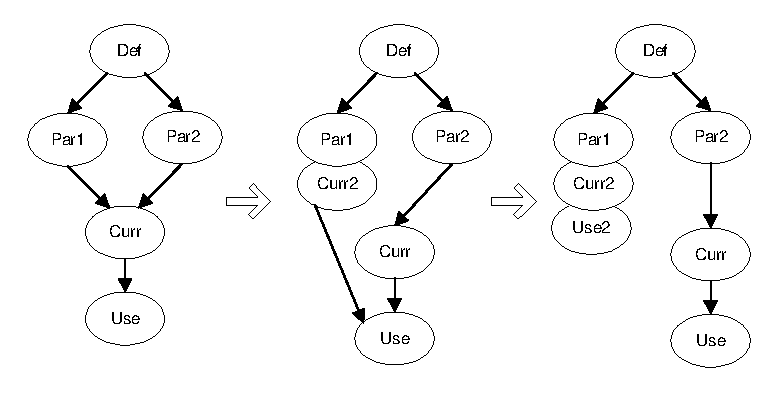
\includegraphics{figures/DuplicateBB.eps}
\centerfigend{fig-duplicateBB}{Duplicating BBs to ensure that each use of
a BasicBlock has a unique definition}

\subsection*{Duplicating a Basic Block}
When the parent of a basic block that needs to be duplicated is a fall-through
or a one-way jump BB, there is only one in-edge, so the RTLs for the current
BB are merely copied
to the end of the list of
RTLs in the parent BB. The parent BB then becomes the same type as the copied
BB, and has the same number of outedges. (The outedges are copied explicitly).
Copying of BBs is done with the clone() member function, to ensure ``deep''
copying. Otherwise, only the pointers to expressions are copied, not the
expressions themselves, and there will be problems when the expressions are
deleted (since the same expression will be deleted twice).

When the parent of a basic block that needs to be duplicated is a two-way BB,
the above method is not suitable. Instead, a new BB is created that is a clone
of the current BB, and the out-edge from the parent to the current BB is
changed to point to the new BB. (Note: this could be the first or ``true''
outedge, or it could be the second or ``false'' outedge). The back end must not
pay attention to the destination of the branch (which remains a faithful
decoding of the original source machine instruction), but rather to where the
BB that the out-edge points to.

In Figure~\ref{fig-duplicate-2way}(a), BB ``Curr'' has a parent BB (``Par1'')
which is a 2-way BB. In this case, a copy of ``Curr'' called ``Curr2'' is made
(Figure~\ref{fig-duplicate-2way}(b)), and the out-edge that used to point to
``Curr'' is changed to point to ``Curr2''. As before, this causes ``Curr2''
to have only one parent, but the successor of both ``Curr'' and ``Curr2''
(the BB ``Use'') now has two parents. When the process is applied to that BB,
we end up with the situation in Figure~\ref{fig-duplicate-2way}(c) where both
``Use'' and ``Use2'' have single paths to the defining BB (not shown).

\centerfigbegin
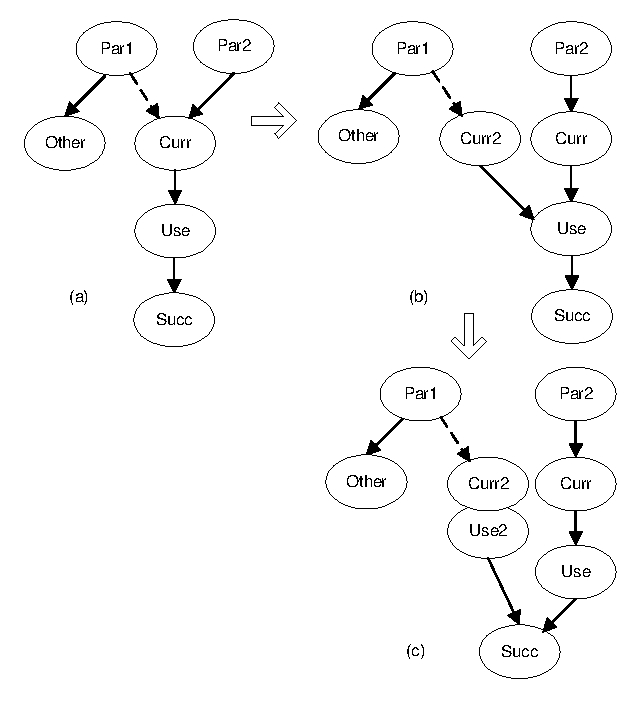
\includegraphics{figures/DuplicateBB2.eps}
\centerfigend{fig-duplicate-2way}{Duplicating a BB with a 2-way parent BB}


\section{Combining Uses and Definitions of Condition Codes}
\label{sec-comb-use-def}

Once unique pairs of CC uses and definitions are found, they must be converted
to a high level equivalent form.

\subsection{Conditional branches and set instructions}

Instructions defining the condition codes are divided into two classes:
``add-like'' and ``subtract-like''. The last RT of the RTL defining the
condition codes (which is expected to be an RTFlagCall\footnote{An object of
class RTFlagCall represents a call to a function that nominally sets the
condition codes for a family of instructions. For example, LOGICALFLAGS sets
the flags for the logical family of instructions.} object) is examined. If
the strings ``SUB'' or ``FFLAG''\footnote{Floating point compares are
considered to be always ``subtract like'', and SETFFLAGS is a typical
flag call function name for setting the floating point condition codes.}
are found in the name of the flag call function, the
instruction defining the condition codes is classified as ``subtract-like''.
Examples include compare instructions, and actual subtract instructions.
Otherwise, the instruction is classified as ``add-like''; examples include
logical instructions such as AND, multiply instructions, and actual ADD
instructions. It is therefore important that the flag call functions are
named appropriately in the SSL file (see section~\ref{sec-srd} for details).

Subtract-like definitions are handled by constructing a high level comparison
expression based on the operands of the comparison or subtraction, and the
type of branch or set instruction. For example,
\begin{verbatim}
 sub a, b, c    # Subtract b from a, result to c
 ...
 sge dest       # Set dest to 1 if "greater than or equals"
\end{verbatim}
has the following high level expression associated with it: ``a $>=$ b''.
The expression is stored in the HLJcond or HLScond object associated
with the RTL that uses the condition code. (The \texttt{setCondExpr} method is
used.)

It is not possible to use the operands directly, since in the final program,
a and b could be modified before the instruction that uses the condition codes.
A mechanism is needed to ``transport'' the condition code information from the
defining instruction to the using instruction. Variables (e.g. ``v12''),
unique to this definition-use pair, are used for this purpose.
Subtract-like definitions of the condition codes
require two such variables; one is needed for each operand.

The variables are copied from expressions passed to the HLFlagCall RT. This
ensures that the correct arguments are copied.

It is important to realise that the result of the subtract is \emph{not}
sufficient to store the result of an unsigned comparison; e.g. v12 = b \gtu\ c
and then branch if v12 \gtu\ 0. For example, 4 \gtu\ 3 and 4-3=1 \gtu\ 0. But
(using 8 bit operands) 204 \gtu\ 3, but 204-3 = 201 == -55, which is a negative
result. (Besides, everything is unsigned greater than 0, other than 0 itself).
The result of the unsigned comparison is in the carry flag, which is a sort of
9th bit of the result.  Therefore, it is not possible in general to save on
variables where unsigned comparisons are involved.

Example pairing:
\begin{verbatim}
10b84:  d0 07 bf e8        ld           [%fp - 24], %o0
10b88:  80 a4 00 08        cmp          %l0, %o0
10b8c:  1a 80 00 04        bgeu         0x10b9c
\end{verbatim}

translates to:

\begin{verbatim}
 v2=*(...);                 # %o0 is mapped to variable v2
 v30=v2;                    # Copy operand 1
 v29=r16;                   # Copy operand 2
 r0=(r16)-(v2);             # The compare, expressed as a subtract
                            #  (result is not used)
 v2=70656;                  # Delay slot instruction
 if (v29 >= v30) goto L11;  # Unsigned comparison
\end{verbatim}

By contrast, add-like definitions need only the result of the operation 
that sets the condition codes. It is an error to find unsigned branches 
or set instructions using the condition codes from an add-like definition. 
For example
\begin{verbatim}
 add a, b, c        # Add a and b, result to c
 ...
 jge dest           # Jump if "greater or equal" to dest
\end{verbatim}
becomes
\begin{verbatim}
c = a + b;
v12 = c;
 ...
if (v12 >= 0) goto dest;
\end{verbatim}

The exception to the above rules are the \texttt{HLJCOND\_JMI} and
\texttt{JLJCOND\_JPOS} branches. These can be used after add-like or after
subtract-like operations (usually a genuine subtract), but since they depend on
the result of the operation, they must be used in an add-like manner.
For example, from
\begin{verbatim}
10bec:  90 a2 20 01        subcc    %o0, 1, %o0
10bf0:  3c bf ff fa        bpos,a   0x10bd8
\end{verbatim}
we generate
\begin{verbatim}
r8=(r8)-(1);
v8=r8;
if ((v8)>=(0)) goto L3;
\end{verbatim}

The analysis code makes the assumptions that the last RT of the RTL defining
the condition codes is a flag call, and (for the above cases) that the second
last RT is an assignment to the result of the operation defining the flags.
Note that if there is a second branch that depends on the above operation,
the second last assignment will be to v8, but it still has the result of the
operation, so it will work correctly.

For other subtract-like operations and branches, it is assumed that the
first two operands (in order) of the flag call are the two operands being
compared (or subtracted). In other words, after
\begin{verbatim}
  x := y - z
  SUBFLAGS(a, b, ...)
\end{verbatim}
it is assumed that a is y and b is z.

As a result of these assumptions, the user is not free to use unusual
semantics in the SSL file. It is hard to imagine the above assumption not
being valid, but it should be kept in mind. In extreme cases, the result of
the operaton may have to be assigned to a temporary variable, then to
either the true destination or another temporary in the second last RT.

\subsection{Assignments that use Condition Codes}

When the instruction using a condition code is an assignment, it is usually
part of an idiomatic sequence.  Two idioms have so far been found and
implemented. The other class of instruction using the carry flag is as part
of multiword arithmetic (e.g. addcc, addx). It may be practical to implement
the multiword arithmetic pairs when the type analysis is able to cope with
variables in two registers; for now, these sequences generate an error message.
This example is from the Solaris 7 /usr/bin/awk:
\begin{verbatim}
142e8:  d2 07 20 00        ld           [%i4], %o1      # Load high half
142ec:  d6 07 20 04        ld           [%i4 + 4], %o3  # Load low half
...
                           # addcc sets flags according to result; add does not
14330:  b4 82 e0 01        addcc        %o3, 1, %i2     # Add 1 to low half
14334:  b2 42 60 00        addx         %o1, 0, %i1     # Add carry to top half
...
142d0:  f2 27 20 00        st           %i1, [%i4]
142d8:  f4 27 20 04        st           %i2, [%i4 + 4]
\end{verbatim}

Here, there are 64 bit integer quantities in the register pairs \%o1:\%o3,
and also \%i1:\%i2 (the colon represents concatenation).

The first idiomatic sequence is: ``compare 0 to a; use carry flag''. Arithmetic
assignment statements using the carry flag need no extra transformation; they
decode to RTLs which use the \%CF register (machine independent carry
flag). For example, \texttt{addx \%g0, 0, \%o3} decodes to
``r[10] := r[0] + 0 + \%CF''. (In the final C output of the translator, \%CF
is represented by the integer variable CF). Therefore, the only transformation
required is to ensure that each use has a unique definition, and to make an
appropriate assignment to \%CF.

Since subtracting any value from zero will generate a carry, unless that value
is zero, comparing 0 to X is equivalent to setting the carry flag only if X
is non-zero. In other words,
compare 0 to X is transformed to ``\%CF = (X != 0)''. An appropriate
assignment RT (i.e. an object of class RTAssgn) is created, and appended to the
list of RTs for the RTL defining the flags. For example:
\begin{verbatim}
10aec:  80 a0 00 0b        cmp          %g0, %o3        # %g0 is always 0
10af0:  94 60 3f ff        subx         %g0, -1, %o2    # Make use of %CF
10af8:  96 40 20 00        addx         %g0, 0, %o3     # Another use of %CF
\end{verbatim}
transforms to
\begin{verbatim}
         # Variable v5 represents register %o3 for this procedure
00010aec *32* r[0] := -v5           # The compare, expressed as a subtract
         *32* %CF := v5 ~= 0        # Generated assignment
         SUBFLAGS( r[0], v5, r[0] )
00010af0 *32* v4 := -%CF + 1        # Register %o2 is held in variable v4
00010af4 *32* v5 := %CF             # Register %o3 is held in variable v5
\end{verbatim}
In C, this becomes
\begin{verbatim}
        r0=-(v5);
        CF=(v5)!=(0);
        v4=(-(CF))+(1);
        v5=CF;
\end{verbatim}


The second idiomatic sequence is similar: ``compare X to Y; use carry flag''.
This is transformed to ``\%CF = X \ltu\ Y'' (where \ltu\ represents ``unsigned
less than''). After subtracting Y from X, a carry will be generated if and only
if Y is greater than x (with both X and Y considered as unsigned quantities).
In other words, after cmp X, Y the carry flag represents the logical expression
X \ltu\ Y.

\section{Complex example}

Despite the apparent simplicity of the above, real code can be surprisingly
complex. The following SPARC code is from the 126.gcc Spec benchmark, generated
from the last 4 lines of C here:

\begin{verbatim}
  int unsignedp = TREE_UNSIGNED (index_type);
  typedef rtx rtx_function ();
  rtx_function *gen_bgt_pat = unsignedp ? gen_bgtu : gen_bgt;
  rtx_function *gen_bge_pat = unsignedp ? gen_bgeu : gen_bge;
  rtx_function *gen_blt_pat = unsignedp ? gen_bltu : gen_blt;
  rtx_function *gen_ble_pat = unsignedp ? gen_bleu : gen_ble;
\end{verbatim}

The addresses of the eight functions (e.g. \texttt{gen\_bgtu}) are set up in
registers like \texttt{\%i2} and stack memory like \texttt{[\%sp + 144]}
in earlier code that is not relevant to the analysis.

\begin{verbatim}
7834c:  80 90 00 1b        orcc         %g0, %i3, %g0
78350:  02 80 00 04        be           0x78360
78354:  a8 10 00 1a        mov          %i2, %l4
78358:  10 80 00 02        ba           0x78360
7835c:  a8 10 00 19        mov          %i1, %l4
78360:  22 80 00 04        be,a    0x78370
78364:  e4 03 a0 90        ld           [%sp + 144], %l2
78368:  10 80 00 02        ba           0x78370
7836c:  e4 03 a0 94        ld           [%sp + 148], %l2
78370:  22 80 00 04        be,a    0x78380
78374:  e2 03 a0 98        ld           [%sp + 152], %l1
78378:  10 80 00 02        ba           0x78380
7837c:  e2 03 a0 9c        ld           [%sp + 156], %l1
78380:  02 80 00 04        be           0x78390
78384:  90 10 00 1c        mov          %i4, %o0
78388:  10 80 00 03        ba           0x78394
7838c:  a0 10 00 1d        mov          %i5, %l0
78390:  e0 03 a0 a0        ld           [%sp + 160], %l0
78394:  92 10 00 15        mov          %l5, %o1
\end{verbatim}

The orcc instruction at the top is the definition for the following conditional
branch, and also three more branches. Because of the two-way BBs between the
definition and the conditional branches, there are a lot of BB duplications
required to translate this code.

There are also several ``orphan'' basic blocks generated as a result of
untangling the delay slots in the above. The code above generates some
23 basic blocks, as shown in Figure~\ref{fig-complex-example}.

\centerfigbegin
{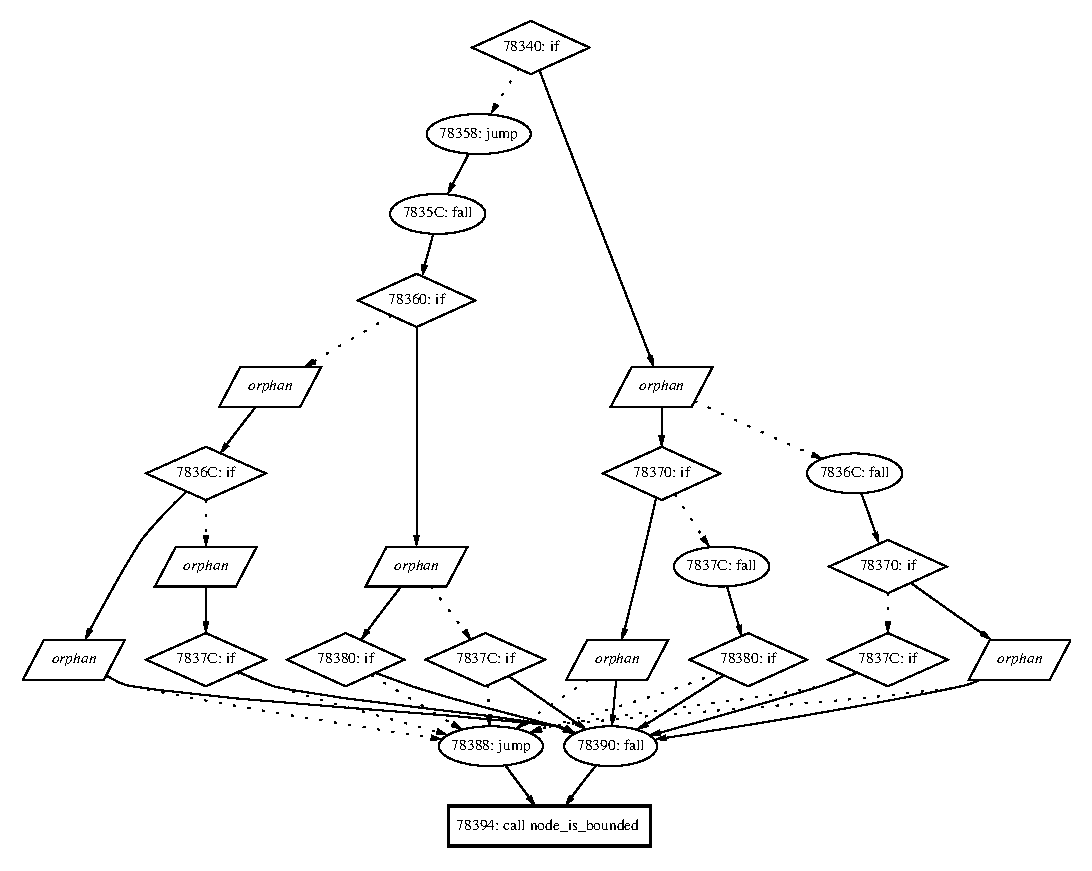
\includegraphics{figures/complex_example.eps}}
\centerfigend{fig-complex-example}{BBs generated for the complex example}
